\documentclass[a4paper,11pt]{article}

\usepackage[top=.8in, bottom=.9in, left=.85in, right=.85in]{geometry} % Don't lower margins more than this, or we might not be able to print it properly

\usepackage[english]{babel}
\usepackage[utf8]{inputenc}
\usepackage[all]{nowidow}
\setlength{\parskip}{2pt plus 1pt}

\usepackage{amsmath,amsfonts,amsthm}

\usepackage{graphicx}
\graphicspath{ {images/} {logos/} {signatures/} }

\usepackage[justification=centering,width=.85\textwidth]{caption} %format=hang
\usepackage{subcaption}

\usepackage{array}
\newcolumntype{M}{>{\centering\arraybackslash}m{1.5in}}
\renewcommand{\arraystretch}{1.5}

\usepackage[colorinlistoftodos]{todonotes}
\usepackage{hyperref}
\usepackage{verbatim}
\usepackage{multirow}
\usepackage{indentfirst}
\usepackage{enumitem}

\newcommand{\horrule}[1]{\rule{\linewidth}{#1}} % Create horizontal rule command with 1 argument of height

\title{
	
\includegraphics[scale=0.4]{logos/bristollogo_colour}\\
	\horrule{0.4pt} \\[0.2cm] % Top horizontal rule
	COMS30400 Report\\
    \Huge The Phoenix Protocol\\
    \horrule{0.4pt} \\[-0.5cm] % Top horizontal rule
    \vspace{1cm}
    % 
\includegraphics[scale=0.4]{logos/bristollogo_colour}\\
    %
\includegraphics[scale=1.0]{bristolcrest_colour}\\

\includegraphics[scale=0.35]{images/pyrolite}\\
}

\author{Dillon Keith Diep, Frank Hemsworth, Marc Steene,\\ 
		Andrei Poenaru, Luke Bryant, Stoil Ganev, Artur Gemes}

\date{9 May 2016}

\begin{document}

\maketitle

\clearpage

\section{Signed Assessment}

\begin{table}[ht]
  \centering
  \large
  \begin{tabular}{|M|M|M|}
      \hline
      Member			  & Weighting & Signature \\
      \hline\hline
      Dillon Keith Diep & 1 & \\
      \hline
      Frank Hemsworth   & 1 & \\
      \hline
      Marc Steene       & 1 & 
\includegraphics[width=.15\textwidth]{marc} \\
      \hline
      Andrei Poenaru    & 1 & \\
      \hline
      Luke Bryant       & 1 & \\
      \hline
      Stoil Ganev       & 1 & \\
      \hline
      Artur Gemes       & 1 & \\
      \hline
  \end{tabular}
\end{table}

\clearpage

\section{Top Ten Contributions}

\begin{itemize}
	\large

  \item Main game networking allowing an arbitrary number of clients and additional networked screens
  \item Infrared motion tracking, enabling pointing and shooting on multiple very large screens
  \item Custom built guns with IR cameras, integrated phone mount and custom triggering mechanism
  \item Development following the Agile methodology, including Agile software (JIRA, git), weekly sprints, epics, stories, and continuous integration following OOP best practices
  \item Infrastructure which allows an unlimited number of spectators to join the game at any point via a web interface which runs on any modern platform, including mobile devices
  \item Different game mechanics and input methods for each role, including a touch screen, infrared controllers, and two different joysticks \todo{change this}
  \item Cutting edge graphics features including physically based rendering and a post-processing pipeline
  \item Custom artwork including 3D models (Maya 2016) and 2D graphics (Photoshop CS6)
  \item Heavily optimised graphics and code, with our target hardware running the game at 60+ frames per second across three game instances at 1024x768 resolution
  \item Self-organised testing and feedback session with CS Department members
\end{itemize}

\clearpage

\section{Abstract}
The Phoenix Protocol is an epic space-fantasy video game where players form a team to survive an onslaught of hostile alien ships as they escape from the fallen Earth. It is an cooperative action-strategy hybrid that encourage players to communicate with one another to decide how best to make use of their abilities and aid their survival. The game is set in a room which forms the bridge of a spaceship with three large back projected screens that surround the players and immerse them into the universe. 
Players take the role of the crew of Phoenix-9, the last remaining human ship capable of intergalactic travel. With Earth on the brink of destruction under the assault of the alien race Glom, humanity faces extinction unless the crew can guide the ship through the portal and reach safety.

There are several roles aboard the Phoenix-9, each playing a unique role in the game:\todo{role repeated twice}

\begin{itemize}[noitemsep,topsep=.5ex]
  \item The \textbf{Commander} is responsible for piloting the ship, which includes dodging asteroids and swarms of enemies. They also have the strategic role of managing upgrades and repairs through the command console interface. This shows useful statistics such as current health and number of resources, and allows the commander to purchase upgrades and repairs for the ship. On top of this, the Commander also has control of a number of powerful abilities, such as engine boosters to quickly escape enemies and rockets to defend the ship if it is in imminent danger. 
  The commander controls the ship's movement via a joystick and manages upgrades, repairs and abilities via a touch screen interface. 

  \item Up to four \textbf{Officers} are each equipped with an infrared gun controller to take down incoming enemy ships. Their mission is to protect the ship from the attackers. A phone display mounted to the top of the gun shows the available ammunition and any incoming notifications for the officer.

  \item Officers also have access to a separate terminal known as the Engineer Console. Once the Commander purchases an upgrade or repair, one of the Officers must put down their weapon and take control of the \textbf{Engineer} and fly it to the appropriate ship part and apply it. This forces the Officers and Commander to strategise and continuously communicate with one another so they are aware of pending upgrades and repairs.
\end{itemize}

\begin{figure}[h!]
	\centering
    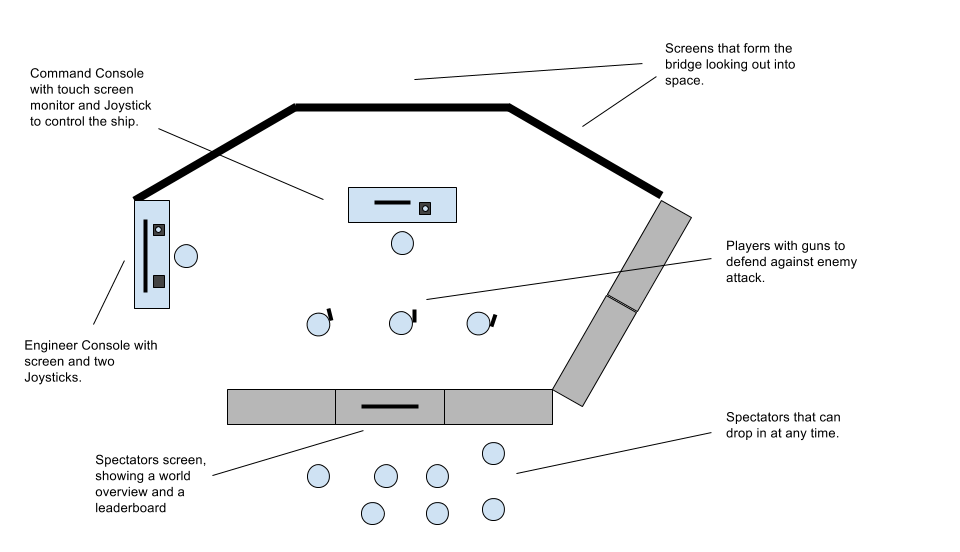
\includegraphics[width=0.\textwidth]{images/roomCropped}
    \caption{The bridge, room layout of of 1.06.}
    \label{fig:room_layout}
\end{figure}

The primary mission is to reach a portal which will transport the ship to safety, away from the alien fleet. Outposts, which house civilians and resources will be encountered on the way. The ship is able to save the civilians stranded on the outpost and collect any resources stored inside. Enemy ships blockade outposts in the hope to foil rescue missions. The players must get past these enemies to save the civilians and collect resources which are vital to upgrading the ship and to be able to reach the portal. 

Spectators waiting to try the game are able to jump into the action and interact directly with the main game through a web page on their mobile device. The mobile game allows them to hack nearby enemies by touching and holding onto enemy sprites in a top-down view of the main game. Hacked enemies can then be controlled, moving to designated locations or attacking other enemies on command. Enemies that have been hacked are visible on the main game and are marked with the spectator’s username to show the players the impact they are having on the game. Spectators compete with each other by gaining points for each enemy their hacked ship kills. A leaderboard is shown on a monitor in front of the players for spectators to see, which encourages competitiveness. The players of the main game are decided by the top ranking spectators after each round. When the current game has finished the top ranking spectators are promoted to the main game and a new team is formed to save humanity.

An immersive environment is constructed by incorporating the physical area into the game. For this project the designated area of demonstration is room 1.06 of Merchant Venturers Building, which was transformed into the interior of the space ship. Multiple screens are utilised to surround the player in the space environment. In addition the use of lights and surround sound are utilised to reinforce the immersive experience for the players and spectators. 

\todo[inline]{Do we need a page break here?}

\clearpage

\section{The Team Process}

From the beginning it was expected of the team to operate in a professional manner. This led to the team mutually agreeing to a number of terms which are detailed in the team contract.

The team followed the Agile development methodology. As such, work was divided in week-long sprints, and regular meetings were held at the start of every sprint to review work, allocate tasks, discuss design and potential issues. During holidays group calls were used in place of physical meetings. This was agreed on the contract and upheld by every member throughout the project.

Initial meetings were largely focused towards the design of the system. After the main components were decided, each team member started working on the one of their choice, according to their interests and prior experience. Subsequent meetings started with a review of each person’s work in the previous sprint and an outlook towards the next one. This was done so that everyone is up to date with all parts of the project, not just the one they were currently working on. The reviews also contained brief demonstrations of the work achieved, so there was constant feedback from the other team members, which helped identify any issues as early as possible. Notes were taken during every meeting to record the progress of the project and to make it easy to review previous meetings, should the need arise to do so. Each member also maintained their own timesheet documenting the tasks completed each day and the time spent on them to ensure a fair evaluation of weightings at the end of the project.

Due to the size of the project, new tasks constantly appeared, and it was likely that cooperation with those working on other parts of the game was needed to solve them. This is because interoperation between components, e.g. protocols, interfaces and REST APIs, had to be agreed on and then tested together. This naturally led to task reallocation and balancing of workload on every meeting, thus allowing everyone to have enough open tasks so there is always something to do, while not blocking other people from their work. This was also a good opportunity for those struggling with their current tasks to ask for help, or request that they work on a different part.

\subsection{Tools}

To track tasks and bugs we used Jira, a well-known and feature-rich issue tracker which provides free community licenses for self-hosting. We were able to host our instance on Digital Ocean, a Virtual Private Server provider, through the free credit from the GitHub Student Pack. Jira acted as the main dashboard where tasks are created, assigned and marked as done, and where possible implications of adding new features or changing existing ones were discussed. It also integrates with Bitbucket, so it can be easily seen which issue a specific change is meant to address. Through using Jira’s issue organisation features, such as task priority and epic links, workload was more easily managed, team members with less to do could be easily assigned new tasks, and the sprint’s features directly guided weekly reviews.

The main communication channel was the cloud-based service Slack. This allowed having a chat environment dedicated to the project, as it was vital that the team kept in touch over the duration of the project. In addition to the messaging, Slack integrates centralised notifications from other services we used, including JIRA, BitBucket, Google Drive, and Google Calendar.

Google Apps provided the main administrative tools we used, including Calendar, Docs for the design specification and notes, Sheets for timesheets, and Drive for file sharing and collaboration with the musicians. The Google suite provides easy sharing with others, which allowed all members’ calendars to always be up-to-date and enable simultaneous editing of files. Google Forms was also used during test sessions for guests to input feedback in a structured manner.

For source control, we used Git. We used BitBucket as the central place to store our repository, from which team members cloned on their development machines. Git allows multiple users to work on the project at the same time, and provides a full revision history of the code, meaning it is easy to see when each change was made, who authored it, and even revert it if necessary. It also allows tagging stable versions, or milestone points, so that there is always a working game available. Using a hosted git repository enabled other team members to review or test code before it was merged into the main release branch.

\begin{figure}[ht]
	\centering
    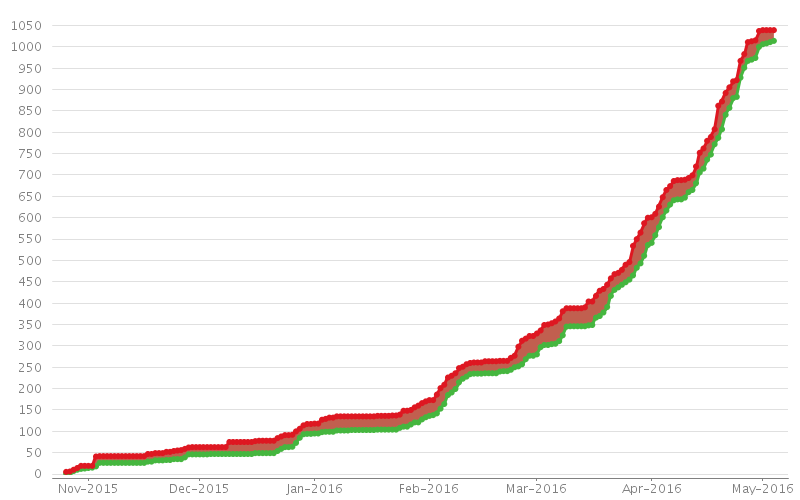
\includegraphics[width=.75\textwidth]{jira_open_vs_closed}
    \captionof{figure}{Plot of open (red) and closed (green) issues for Jira. A spike in open issues can be observed once all components are put together after Christmas, and again after user testing. The curve tails off with only balance left for the last weeks.}
\end{figure}

\section{Project Planning}

\subsection{Time management}
The initial schedule was developed around the main components of the game. The target was to get the main features running as soon as possible, then move on to less critical ones, so that delays were less likely to cause game-breaking problems.

We organised the project into epics, such that each component formed a separate epic. Within each epic, we started with stories that described the expected behaviour of that component. Based on these stories, we produced small-sized tasks.

We set internal deadlines to make sure no component becomes a bottleneck for the whole game, and then development started on most components simultaneously. The spectator game was deemed lower priority, as it was block by the main game. At the highest level, we aimed to have the core gameplay implemented by Christmas, and all the features in the game by Easter.

The first big change to this schedule was caused by switching from a 3-screen game to a scalable network architecture. Initially, the game was specifically designed to take advantage of the three big screens in MVB 1.06, but it became clear around November that it might not be possible to get a powerful enough machine to run the game - there were also concerns regarding the camera distortion of a wide viewing plane due to the non-linear positioning of each projector screen in MVB 1.06. At the same time, due to issues with the projectors and the lack of response from IT Services, we decided to take a new approach which allowed us to use any number of screens, as well as split the rendering load across multiple machines. This took the form of the networked-multi-screen architecture which is present in the final game, and the deadline for which was Christmas.

Partly due to our regular meetings and use of sprints to measure progress, we mostly followed the initial schedule. The networking was done before Christmas, and the game was playable, although almost all assets were placeholders and only the mouse and keyboard controls could be used. However, because more than half of our team had 70 CP of units in the first term, not as much was accomplished as initially planned. At that point, the command console was underdeveloped, and gun shooting was not implemented.

Fortunately, after the exam period we made steady progress, and more gameplay features were added. We also began replacing the placeholder graphics and assets with the final versions. The engineer was also in a near-final state soon after. We were now in a position to start focusing on the spectator game and integrating more gameplay elements with the different player roles.

This advanced neatly, and around Easter we had a feature-rich game that was not missing any vital part, but lacked polish. It was also not very user friendly, with little to explain the aiming and mechanics of the game, which would become the focus for the last part of the project.

After Easter, significant improvements were made to the command console and the gun shooting. The spectator game was also finalised, and by the time we got users in for a proper testing session, the game was in good shape.

However, as expected, the testing session, which involved several members of the Department, brought several issues to our attention regarding the game’s atmosphere and general user-friendliness. We aimed to address these issues before the Games Preview Day, which required constant play-testing and balancing. After this point, everything was in place with only a handful of bugs to fix.

\todo[inline]{Mention internal testing day and show some results of feedback form (they were all very positive, ref difficulty users praised ease)}

No major feature was developed in the last two weeks of the project. We had aimed to use this time just to fix bugs and test the game extensively, which in doing so we gained confidence that our game would perform well on Games Day and that it was unlikely to encounter bugs. Most remaining bugs after the Preview Day were fixed within three days, and the rest of the time consisted mainly of testing and small balance tweaks.

\todo[inline]{Add more about actual deadlines and milestones}

\subsection{Collaborators}
\todo[inline]{Full names of Musicians?}
We worked with students from the Music department (Lefteris, George and Tom) who composed the music for our game. We first met them during the initial composers meeting before Christmas, when we explained to them the main idea of our game. After the holidays, we met and decided what type of music we wanted, and how many tracks. They then composed and produced our music, giving us various opportunity to give feedback on their work, which meant we could make sure we obtained exactly the kind of music that we had envisioned for the game. Although initially they said they were able to help with sound effects as well, due to time constraints on their part, we did not use sound effects created by them in the project. 

Our mentor, Andrew Stubbs, was also a part of our development process. We met with him several times over the course of the year to keep him up-to-date on our progress and obtain feedback. In our first meeting in autumn, he told us about his experience with the Games Project from when he was an undergraduate several years ago. Most of his advice was centred around time management and task distribution, which again showed how serious we would need to be about these issues. In the following meetings, we continued to show him our progress and ask for his opinion the current state of the game, as well as any outstanding design decision. We invited the mentor to our self-organised testing day, where he spent a lot of time playing the various parts of the game and giving us in-depth feedback. Working with him has been a great experience for us, and his advice has been invaluable to our good progress.

We also worked with the voice actor Jordan Woollen who provided the voice of the Admiral. We made a post on a forum where voice actors provide free work and were lucky enough to receive several auditions from voice actors enthusiastic about our game.

\section{Documentation}

\todo[inline]{Decide if we're including this here: Show how you maintained your software during its development.}

\subsection{Running the game}

First, the screens need to be set up. For each screen, one instance of the game needs to be run. Then, the commander and engineer consoles each need a separate client as well. The default option is to have the server run the middle screen, then join with the side screens as clients, but this can be easily changed after the clients have been connected. The IP address of the server needs to be entered in the text field in the top right-hand corner of the main screen. When the server has been started, the IP address is displayed in the lower right-hand corner of the screen. Making sure all the clients are connected, press \texttt{Start}. Figures \ref{fig:first_screen} and \ref{fig:lobby_screen} show screen shots of the setup screens.

\begin{figure}[ht]
	\centering
    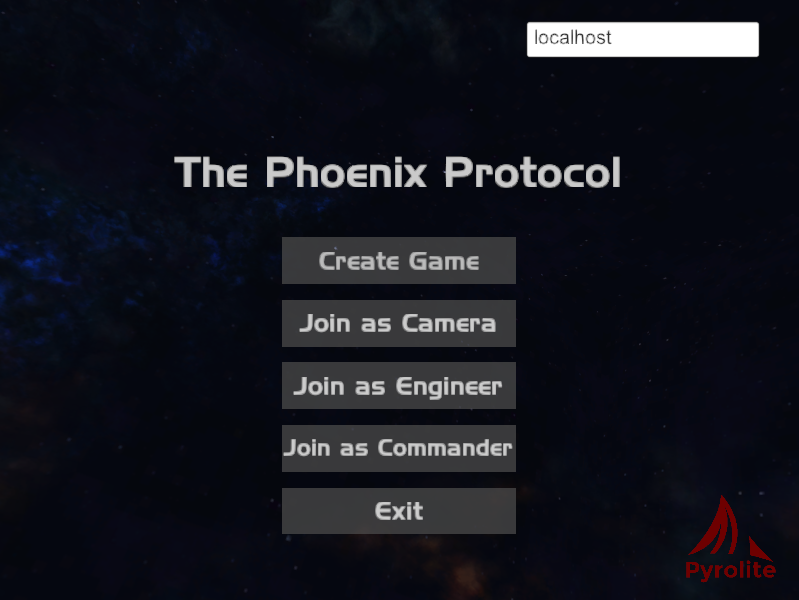
\includegraphics[width=.7\textwidth]{game_first_screen}
    \caption{The main screen of the game. The IP address of the server is entered in the the text field at the top, and client roles are selected using the buttons.}
    \label{fig:first_screen}
\end{figure}

\begin{figure}[ht]
  \centering
  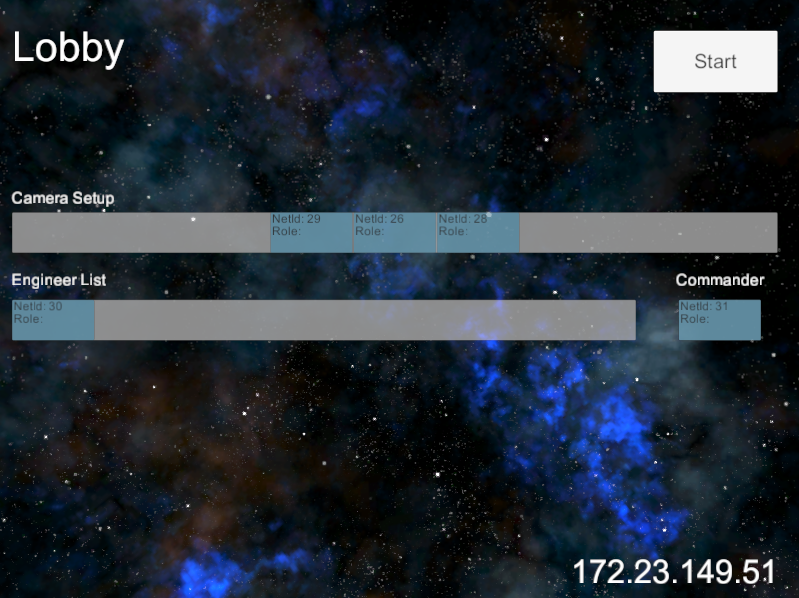
\includegraphics[width=.7\textwidth]{game_lobby_screen}
  \captionof{figure}{The game lobby screen with all clients joined in their specific roles, as seen from the server. The IP address is shown in the bottom right.}
  \label{fig:lobby_screen}
\end{figure}

Next, start the phone server by providing it with the game server IP using the \texttt{-ip} flag. This will also allow you to open the admin panel. By default the admin panel can be accessed through a browser on port \texttt{52932} at the address of the phone server. At this point, players can join the game with their phones. When everyone has joined, use the admin panel to assign roles to the players, then start the game when ready. This will start all components of the game. Figure \ref{fig:admin_panel} shows a screen shot of the admin panel.

\begin{figure}[ht]
	\centering
	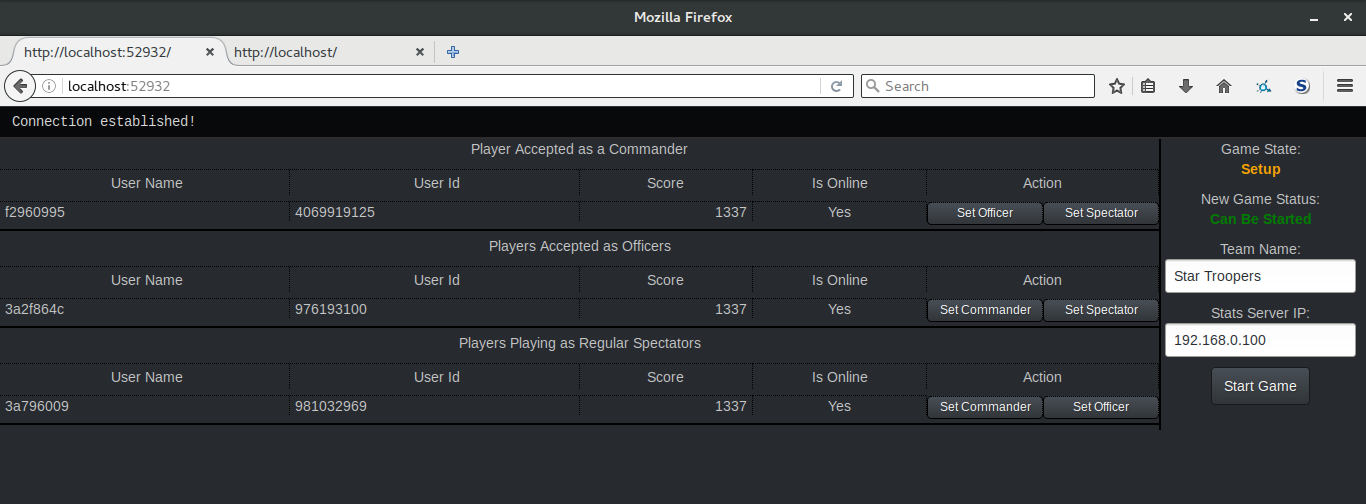
\includegraphics[width=\textwidth]{images/admin_panel}
    \captionof{figure}{The admin panel. The user can set player roles and specify a team name during the setup stage of the game.}
    \label{fig:admin_panel}
\end{figure}

\subsection{Extending the game}
One of the strong points of our design is its modularity. In this sense, the main interaction components, such as the gun controllers or the networked multi-screen architecture, are almost completely independent. It would be easy to extract these components and plug them into a new, completely different game.

The screen positioning and camera angles and field of view can also be changed by simply altering a set of parameters. Thus, it is easy to obtain the desired configuration of number of screens and field of view, without having to change any of the code. The existing system also accounts for a user-defined size of dead space between the screens, which again helps with positioning in a new environment.

While the infrared aiming is tuned for three screens, it would not be difficult to introduce more screens. The same algorithm used in our game could be applied to any number of distinct patterns, and as long as there is one pattern per screen, the system would work without any changes in logic.

The graphics is completely modular as well, so a visual makeover would not need to change any of the existing code. This includes 3D models, 2D UI components and tutorial graphics.

Because the project was developed under a git repository from the very first line of code, it is possible to revert to any previous version. It is also possible to find exactly which team member implemented a particular feature, or made a change to specific file.

\todo[inline]{-Good ideas that we wanted to do but no time: ??}
\todo[inline]{There is some overlap here with the Team section}

\clearpage

\section{Technical Content}
\subsection{Networking}

\begin{figure}[ht]
	\centering
	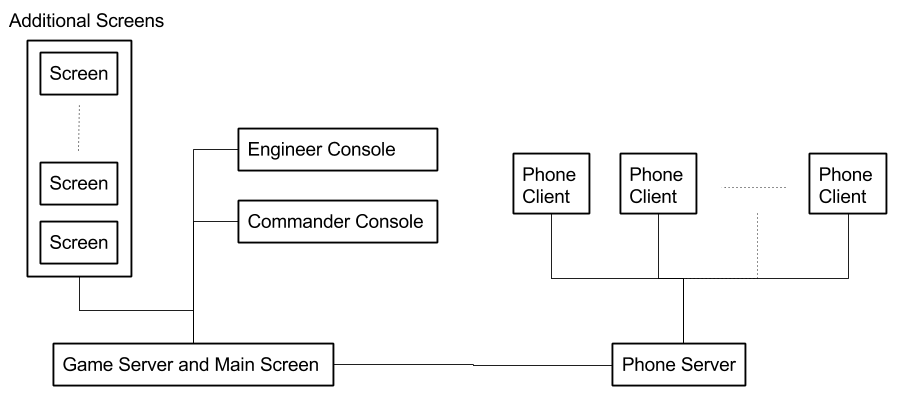
\includegraphics[width=\textwidth]{images/network_diagram}
    \captionof{figure}{An overview of the connectivity between the different components of our game}
    \label{fig:network_diagram}
\end{figure}

Networking is a central part of The Phoenix Protocol, being at the core of both the screen technology and the multi-role system. Networking is done on three main levels:

\begin{itemize}
	\item Between Unity clients, i.e. the main game server, the side screens, and the commander and engineer consoles:
    
	\begin{itemize}[topsep=0ex]
      \item \textbf{Synchronized variables} are used to automatically push game state changes from the server to the clients. These are built into Unity and allow low-overhead synchronisation of the main game logic.
      \item A \textbf{message passing system} implemented using a combination of Unity’s  \emph{Remote Procedure Call} and \emph{Command} systems together with traditional message objects sent using the low-level API. Most of the player actions, such as shooting, ship upgrades and repairs, and commander abilities are implemented this way.
  	\end{itemize}
    
	\item Between the main Unity Game Server and the Phone Server:
    
  \begin{itemize}[topsep=0ex]
 	 \item A \textbf{TCP-based communication channel} is used to send the signals that start, end, or reset a game. It is also used to communicate persistent data such as players scores and game statistics that need to be reliably sent to the database.
 	 \item A \textbf{UDP-based channel} facilitates the synchronisation of game objects between the main game and the spectator game, as well as transmitting back the commands received from the phone clients. In this case, low-overhead is preferred over reliability, since most of these messages are sent many times per second, so the occasional lost packet will not impact gameplay in a noticeable way.
  \end{itemize}
  
\item Between the Phone Server and the phone clients:

  \begin{itemize}[topsep=0ex]
  	\item A single \textbf{WebSocket connection} is maintained per player between a phone client and the Phone Server. This connection is used to send only relevant game data to a phone client and in a format that can be immediately used by the client. Also, clients can send back player related data and actions in order to be later relayed back to the game server. A system is in place to ensure that each player has only a single client associated with it.
  \end{itemize}
  
\end{itemize}

From the above, it is clear that the game needs access to a fast network with low noise. To implement this, a separate LAN was set up just for the game.

\todo[inline]{Maybe add more details?}

\subsection{Player Shooting}
This section describes how the player shooting was implemented. It was decided that a ‘point and shoot’ mechanism for the players would be best. Several solutions to the problem were proposed, the first was to use a camera on the end of the guns with coloured points around the screens that the camera could detect and then determine the position the gun was pointing at on screen. The second, an improvement on the first, was to mount an infrared (IR) camera on the front of the gun and use IR LEDs to determine the pointing position. 
The second solution seemed like the option that would be less susceptible to error, dealing with only blobs rather than having to do image processing greatly simplified the task. Initially a small IR camera was thought to be the solution, but it became immediately obvious that a cheaper alternative would need to be found. The Nintendo Wii Remote\cite{wiibrew_wiimote} has an IR camera on the end and has a large open source community that has reverse-engineered the commands sent over bluetooth. This seemed like an affordable solution to our problem, with the added bonus of the Wii remotes buttons and internal accelerometer. 

\subsubsection{Pointing Position}
The first problem to solve was how to determine where the gun was pointing on the screen. The solution the Nintendo Wii uses is to mount a pair of IR LEDs to the top of the screen. These LED Bars that come with the Nintendo Wii proved to not be suitable for our target setup. The original LED bars are designed for small screens in small rooms. The target room is large and uses very big back projected screens. Custom LED bars were made for each screen with brighter LEDs placed further apart to compensate for the screen size. The pointing position is then calculated by finding the midpoint of the two LEDs and reflecting the point about the middle of the image. For example a point in the bottom right would correspond to a pointing position of the top left on the screen. 

\subsubsection{Field of View}
\todo[inline]{Format equations}
The IR camera that the Wii remote provides has a vertical field of view of 23 degrees, this was a problem for the room, the max distance from the screens is around 350 cm. With this field of view that gives us a vertical view distance of around 148 cm (2*350*tan(11.5)), with a screen height of 180 cm. The field of view was not quite wide enough to see the LEDs at the top of the screens when the player aims to the center of the screen. This issue was solved by mounting the IR camera at an angle on the gun (see right diagram in the figure below).


\includegraphics[scale=0.5]{ir}


\subsubsection{Shooting at Multiple Screens}
To successfully create a point and shoot experience on multiple screens, a method of differentiating the screens was needed. The first solution was to create a third IR LED for each screen that flashes at different frequencies for each screen. This was quickly proved to be impossible due to the refresh rate of the IR camera in the Wii Remote. The Wii Remote can detect up to 4 IR LEDs in a single frame, each screen uses two LEDs to determine the pointing position. This leaves 2 LEDs for each screen to differentiate them. The method that was used was to use three LEDs on the left and right screens and two LEDs on the middle as shown in the diagram below. 

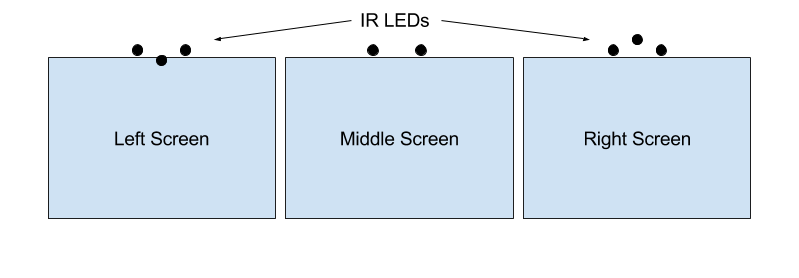
\includegraphics[scale=0.5]{led_pos}

Various challenges were involved when trying to calculate which screen the player is aiming towards. Mainly issues arose around the transitions between screens, for example if the IR camera detected LEDs from different screens the simple rule set would fail and return an erroneous result. 


\subsubsection{Physical Guns}
\todo[inline]{Show how guns were created, feedback from testing…}

\subsection{Multiple Camera System}
A defining feature The Phoenix Protocol is the usage of multiple screens. The simplest solution other games adopt is to use a very wide window that stretches across connected monitors. It became evident that we required a more sophisticated solution as a single large window is expensive to render and inflexible for future consideration, neither is it possible to have the view wrap around by simply increasing the field of view. After the prototyping stage, it was clear that a networked solution of aligned cameras fit the requirement better.

The Unity camera component\cite{unity_camera} uses a set of parameters, most notably the field of view, to define its view of the game world. A view frustum\cite{unity_frustum} is the truncated pyramid that contains the area observable by the camera. The height at a given point is given by Equation \ref{eq:frustum_height}.

\todo[inline]{Add missing pictures}

\begin{align}
	Frustum Height\cite{frustum_equations} = 2 \times Distance \times \tan(Field Of View \times 0.5 \times (\frac{\pi}{180}))
    \label{eq:frustum_height}
\end{align}

Using the frustum height, the width is retrieved by Equation \ref{eq:frustum_width}.

\begin{align}
	Frustum Width\cite{frustum_equations} = Frustum Height \times Camera Aspect
    \label{eq:frustum_width}
\end{align}

Since the desired alignment only requires horizontal rotation, vectors representing the left and right edge of the frustum can be defined using the frustum height.

\begin{equation}
	OF = f
	\label{eq:dillon_stuff_1}
\end{equation}

\begin{equation}
	FL =\frac{Frustum Height}{2}
    \label{eq:dillon_stuff_2}
\end{equation}

\begin{equation}
	OFR = OF + FL
    \label{eq:dillon_stuff_3}
\end{equation}

Using the symmetrical properties of the camera we can derive the right side by Equation \ref{eq:dillon_stuff_4}.

\begin{equation}
	OFL = OF - FL
	\label{eq:dillon_stuff_4}
\end{equation}

The rotation that aligns the left vector to the right is the angle required for aligning cameras. In addition to this, a gap may be included by multiplying the rotated angle by a percentage to accommodate borders between screens in the real world. As the frustum is also affected by the aspect ratio of the program window, camera alignment is performed in setup phase during runtime. A client that is given the role of a camera will then apply the rotation, multiplied by the client camera index for correct positioning.

The solution was extremely well received by testers. The virtue of this scalable solution simplified development as extra screens can be added flexibly. It is possible to use this system to display a 360 view around (and more), or even extend the view vertically.

\todo[inline]{screenshot of 5 cameras}

\subsection{Enemy AI}
The enemy ships use an efficient behaviour control system. Because of the large number of enemies, together with the need for them to be synchronised over the network, a strategy that makes good use of resources was needed. The solution adopted is a swarm-based system that uses randomness and a sequence of state transitions to give the impression of the player being constantly assaulted by fighter-type crafts. 

The enemies have various states which dictate whether they try to engage the player, boost to get in range, or protect an objective, such as an outpost. They are able to engage the player through a set of randomly-generated \emph{waypoints} around the player ship. The enemies constantly choose a random waypoint from their set to visit next, and shoot at the player if in a good position to do so. The forward speed and turning speeds of the enemies have been tuned so that their behaviour appears to be typical of a dogfight, which is helped by the large number of enemies usually present on screen. This strategy has been chosen because it provides a great balance between using few resources and producing great visual results.

The states depend on the enemy’s type and its current relation to the player. Enemies can have 4 \emph{purposes}:

\begin{itemize}[noitemsep,topsep=.5ex]
	\item \textbf{Outpost guards} wait around the outpost they protect until the player comes within range, at which point they engage the player
	\item \textbf{Suicidal enemies} try to crash into the player to damage their ship. To give the player a chance to fight back, enemies are required to enter the player’s field of view before crashing into the ship
	\item Enemies that have been \textbf{hacked} via the spectator game follow the commands sent over from their controller. Their main use is to attack other enemies.
	\item All \textbf{other enemies} try to get in range of the ship, then move around it following the waypoint system, while shooting at the player when at a good angle.
\end{itemize}

The enemies also use an object avoidance system which allows them to go around asteroids, other enemies, or other spaceships such as the Glom Mothership. This is based on ray casts and integrates with the waypoints system to temporarily direct the enemy to a new direction if it detects an obstacle.

Enemies that have been hacked through the spectator game move to a special state where they are able to follow commands given by their controller, and even attack other enemies. This also plugs into the waypoint systems, showcasing its flexibility and supporting it as a good design choice.

\subsection{Spectator game}
While waiting to play the main game, spectators can join the team currently playing by using smartphones. To connect, a spectator needs to join the game’s dedicated WiFi network, then either scan a QR code or type the address of the game’s web app manually. They then get a top-down view of the game centred around the player ship, with objects around it displayed using 2D sprites.

Enemies can be hacked by placing a finger on them and following their movement for a short period of time. If the enemy goes too far from the finger’s position on screen, the hacking progress is reduced, requiring more time until the enemy becomes successfully hacked. Once done, the enemy will follow the player’s ship and wait to be issued commands. On the main game screen, the enemy will be highlighted by a green target (instead of red for non-hacked enemies), and the hacker’s name will be displayed above it. This raises awareness that this particular enemy ship on the player’s side, and allows subtle, if indirect, interaction between the officers and the commander currently playing and the spectators waiting.

Hacked enemies can be ordered to move relative to the player’s ship. Movement uses the same waypoint system as the main enemy AI, including the object avoiding system, which allows smooth integration between hacked and non-hacked enemies. They can also be ordered to attack another enemy ship, which they will follow and shoot at following the same system used when targeting the player. There is, however, one slight difference: suicidal enemies, which cannot normally shoot, are allowed to shoot while hacked. This was implemented because making the hacked suicidal enemies crash into their targets was confusing for players, as it is difficult to tell what type of enemy was hacked based on the sprite on the phone. Additionally, when an enemy is hacked, their bullet damage is tweaked slightly, as the game could seem unfair for a spectator that hacks a very easy or very advanced enemy without being aware of it. This way, all hacked enemies do the same damage per shot, a value which was tweaked to create a dynamic and engaging game for the spectators.

One of the main problems we had to solve for this component of the game was the rendering of the game objects. Initially we considered using Unity as a natural extension of the main component of our game. However, we realised that this would either require from a user to install the Unity Web Player or use a still experimental WebGL based version of the Unity Engine. This would either put off users from playing the game or simply make it incompatible with a significant portion of mobile devices. This is why we decided to investigate a solution based on Javascript and HTML5 Canvas\cite{html5_canvas} since that would be supported by most modern mobile browsers. After some careful consideration we decided to build the spectator game around Pixi.js\cite{pixi_js} as a rendering engine. Pixi.js provides an easy to use API build on top of the HTML5 Canvas and WebGL APIs that allowed us to easily render 2D sprites in a 2D scene. We decided to rely on this library since it allowed us to easily support any size screen, render at a high frame rate efficiently and do simple animations. This might not have been possible within the time frame of this project, if we decided to use the raw HTML5 Canvas API.

\subsection{Phone Server}
The Phone Server is the main mediator between the Game Server and the phone clients. Its main responsibilities revolve around maintaining stable communication channels with the Game Server and the phone clients, passing the necessary data between the Game Server and the phone clients and converting data in an appropriate format before passing it on.

The Phone Server attempts to provide some basic form of connection recovery when the connection to the Game Server is dropped. It this by attempting to re-establish the connection at regular periods of time until it is successful. While there is no connection any internal operations or state transitions that are dependant on communication with the Game Server are blocked. In regards to the phone clients, the Phone Server maintains only a single connection per player. If a new connection associated with a player is established, the old one is dropped and all communication is done through the new one. There are a few reasons why this behaviour was implemented. The first one is that this prevents a user from opening multiple tabs in their browser and forcing the server to serve multiple clients on the same device. Since each tab is considered a separate client, each of them would need to receive updates about the game state. Therefore, a malicious user could simply open a large number of tabs and block a large amount of the servers outbound bandwidth. Another reason for this design choice is the fact that a connection might persist even if an error occurs on a client. Therefore, if a user tries to refresh the spectator game web page to fix a problem, either two connections would have to be handled or simply the new one would have to be blocked. By dropping the old connection instead of the new one, we prevent this case where a faulty client connection persists and prevents any attempt from the user to rejoin.

The spectator game view of the game world is significantly different from the one seen on the main screens and in a sense much simpler. For example on the main screens we are displaying objects in a three dimensional view, while on the phone clients we are displaying them on a two dimensional plane. This means that we have to convert the coordinates, orientation and scale of each object form the 3D plane of the game world into a realistic 2D view suitable for the phone displays. We decided to do this conversion on the Phone Server rather than individually on each phone client for a number of reasons. One of these reasons is that less data would have to be sent to each client. This is due to the fact that a lot less information is needed to display an object in the 2D view rather than in the 3D one. Moreover, the conversion process can be quite costly depending on the number of objects that need to be shown and due to this some older devices might not have been able to handle it. As for the nature of the conversion process, it is an orthogonal projection of every game object onto the plane that intersects the player ship and is parallel to the ship's forward and right directions with its origin set at the location of the ship. In simpler terms it generates a top-down view of the player ship and the objects around it that is centered around the ship itself.

There are multiple reasons as to why we decided to separate the Phone Server from the Game Server. One of them is the fact that, if one of the two components encounters an error and crashes, we can easily restart it without affecting the other. For example if the Phone Server went down that would only cause the disruption of the spectator game without interrupting the players in the main section of the game. Also, this allows us to attempt and fix any problems in the Phone Server while a game is running, without introducing a significant downtime between games. Another reason is that the Game Server performs a significant amount of computation and there is the possibility that the machine it is running on might not be able to handle serving the phone clients. By having the Phone Server as a separate application we can run it on a separate machine and thus distribute the overall computation cost of the system between multiple machine. Unfortunately, this comes at the cost of communicating the game state data between the machines. However, considering the amount of computation in comparison to the communication overheads, we decided that this is a beneficial trade-off.

\subsection{Optimisation}
Sixty frames per second (FPS) is the gold standard frame rate for video games as it produces very smooth visuals and allows almost immediate feedback to user input. For our game, this presented a serious challenge - our plans were ambitious, with hundreds of enemies and bullets, and thousands of asteroids all running simultaneously. On top of this, due to hardware availability, we needed to have three game instances running on the same machine, all rendering at a resolution of 1024 * 768 at 60 FPS. Even with the powerful hardware provided, optimising the game to run smoothly was a challenge.

Unity comes with several built in profilers for the CPU, GPU, memory, physics, and more. These were imperative in our optimisation effort, the profiler provides a breakdown of how much time is spent computing each script or rendering each object, enabling the least performant ones to be identified.

\begin{figure}[ht]
	\centering
	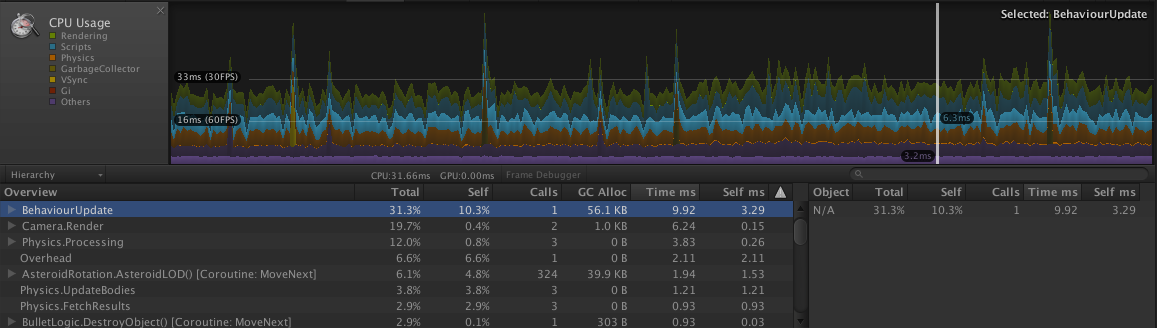
\includegraphics[width=\textwidth]{images/profiler}
    \captionof{figure}{CPU Profiler showing frame composition}
    \label{fig:profiler}
\end{figure}

\subsubsection{Networked Object Pooling}
During the game, multiple objects need to be spawned at run time, including asteroids, enemies, bullets and explosions. Initially, these objects were created at the time of request via instantiation. Instantiation creates a new object in memory and adds it to the scene. This is not an issue when spawning only a few objects. However, it was apparent that this would not suffice our game requirements. Furthermore, each object was destroyed via a Destroy call. When a Destroy call is made on an object it is sent to the garbage collector which releases memory at regular intervals. Due to the volume of objects and memory that needed to be removed, there were regular spikes seen in the profiler that caused reductions in frame rate which appeared as jarring on screen.

To solve this an object pooling system was created. During the loading period at the start of the game, a predefined number of objects are instantiated, for example, 500 bullets. When a script requests a bullet, rather than instantiating a new bullet, an inactive bullet in the object pool is returned for the script to use. Then, rather than destroying the bullet at the end of its life, it is disabled and returned to the object pool for re-use. This eliminated the CPU spikes caused by allocating and freeing memory, resulting in a much smoother experience. Although this was a relatively straightforward implementation on the server, getting it working correctly over the network was more difficult. 

Previously, when an object was instantiated on the server, a function could be called that would create the object on the client and Unity would handle synchronisation. Now that we were simultaneously spawning thousands of objects the network became unusable with extremely high latency. 

To solve this, we created our own implementation of network object spawning to allow networked object pooling while avoiding Unity’s synchronisation. Our implementation removes the direct relationship between server and client objects and allows one object in the server pool to be coupled with an arbitrary object in the client pool, so long as it is available. We then use Remote Procedure Calls and a custom interpolation implementation to synchronise the transform of each object across the network. By doing this, only active objects are synchronised across the network, and due to the object pool implementation, there are very few memory and garbage collection slow downs giving the best of both worlds.

\subsubsection{Network Optimisation}
Synchronising the thousands of objects in our game each frame across the network is not feasible, so we have implemented some optimisations to reduce the load on the network. One example of this is the client predication. A bullet on the client only needs two messages to synchronise correctly with the server - the starting position, orientation, and speed, and another when it is destroyed. As the bullet travels in a straight line, the position doesn’t need to be constantly synchronised and can be calculated on the client. This is also used for the asteroid rotations. To maintain server authority, no collision or logic is performed on the clients.

\subsubsection{Graphics Optimisation}
With thousands of objects within the camera frustum at any time, the GPU was having to draw up to five million polygons at a time, resulting in a low frame rate on our target hardware. Unity comes with frustum culling which removes objects outside the camera view and far plane culling, which removes objects beyond a certain distance. On top of this, we implemented a custom level of detail system for the asteroids. Each asteroid has three different models with varying amounts of detail. Each asteroid calculates the distance to the camera position and swaps out the model accordingly, with lower detail models being used for more distant asteroids. This can potentially reduce the polygon count by 93\% for 2,000 asteroids.

\subsubsection{Script Optimisation}
We have implemented many optimisations across our codebase to reduce computation time as much as possible. One example of this is the targets drawn over enemies - rather than using Unity’s built-in GUI system to render the targets which can be slow, we instead apply the target to a transparent 3D plane that faces the camera, allowing them to be rendered much quicker. We also update the rotation of the plane less as the distance to the player increases as the difference in rotation will be less noticeable. On top of this, we split up large operations across several frames to reduce sharp decreases in the frame rate, for example, when spawning an asteroid field.

Our optimisation effort was very successful, and we can render three 1024 * 768 games instances at several frames higher than our target frame rate.

\subsection{Graphics}

\subsubsection{3D Art}
All 3D models in our game use an advanced lighting model called Physically Based Shading which attempts to mimic a physically correct interaction between light and materials. This offers a huge visual improvement over older Lambertian and Blinn/Phong models, and is implemented in Unity 5’s standard shader.  Additionally, the majority of models in our game use 2048 * 2048 pixel texture maps for the diffuse textures, which adds colour information to the model, and normal map textures, which are a cheap way of adding additional detail to a model without adding more complex geometry. Below is a set of models created by various team members.

\begin{figure}[ht]
	\centering
	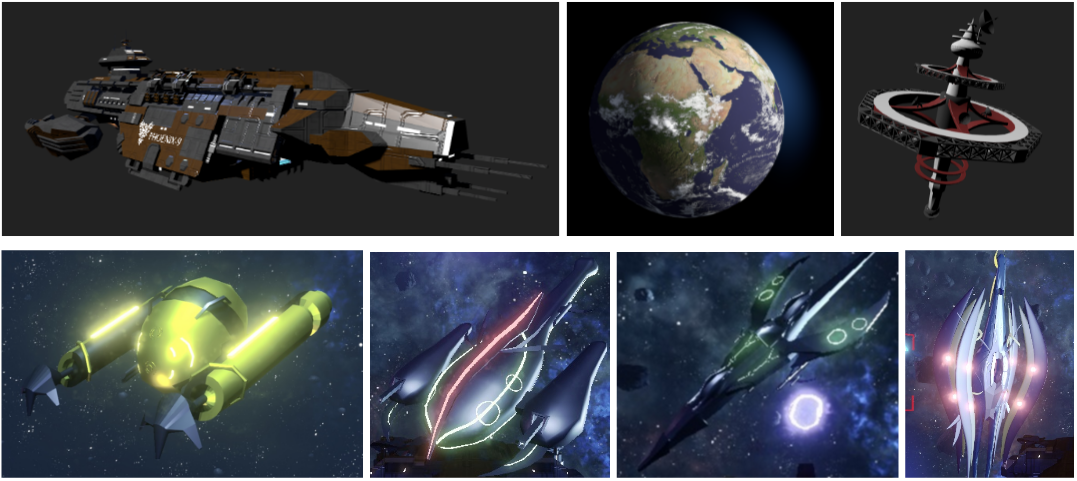
\includegraphics[width=\textwidth]{images/3DArt}
\end{figure}

The Earth object is composed of three layers. The ground and cloud layers use 8192 * 8192 diffuse and normal map textures downsampled to 4096 * 4096. The atmospheric effect is generated from an open source shader that takes into account the direction of the sunlight. The Earth textures have been obtained from NASA’s open source BlueMarble project.

\subsubsection{Rendering Path}
We decided to switch to the deferred rendering mode rather than Unity’s default forward rendering mode. In forward rendering, the computation time is bound to the scene geometry and number of lights - in Big-O notation, the complexity is given by: $O(num\_geometry\_fragments \times num\_lights)$. Our game contains many lights and complex geometry (almost 1.4 million polygons at times) meaning this was not a performant enough solution for our game. On the other hand, deferred rendering has a complexity given as follows: $O(screen\_resolution \times num\_lights)$. By decoupling the amount of geometry from the computational complexity, we are able to render our scene much faster. On top of this, deferred rendering gives us a whole host of other graphical advantages, including HDR enabled cameras, dynamic shadow support for multiple lights, and more complex post processing effects.

\subsubsection{Post Processing}
One of the biggest downsides to using deferred rendering is the loss of support for multisample antialiasing (MSAA). Currently, there is no perfect solution for antialiasing in deferred rendering and it is the subject of ongoing research. Supersampling, where the image is rendered at a higher resolution then downsampled, does remove aliasing but is too computationally expensive for most real time graphics. Thus, we are limited to screen space anti-aliasing methods. SMAA is one of the best available antialiasing methods to date, and we use it in our game to reduce jagged edges. It is more computationally expensive than a simpler solution such as FXAA, but results in less texture blurring.

Bloom is an effect that simulates the bleeding of light when a camera is exposed to a bright light source. Switching to the deferred renderer allows us access to HDR cameras, meaning it is possible to render physically correct bloom. The effect is noticeable on bright elements in the game, such as the sun and glow on enemies.

\begin{figure}[ht]
	\centering
    
    \begin{subfigure}{.5\textwidth}
      \centering
      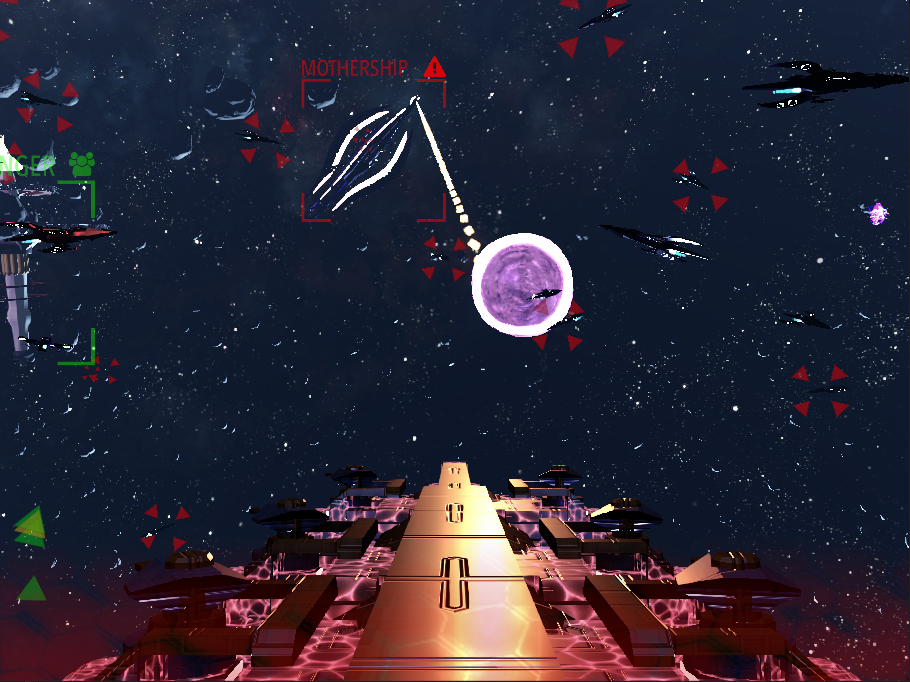
\includegraphics[width=0.9\textwidth]{bloomOff}
      \caption{Bloom disabled}
      \label{fig:bloomOff}
    \end{subfigure}%
    \begin{subfigure}{.5\textwidth}
    	\centering
		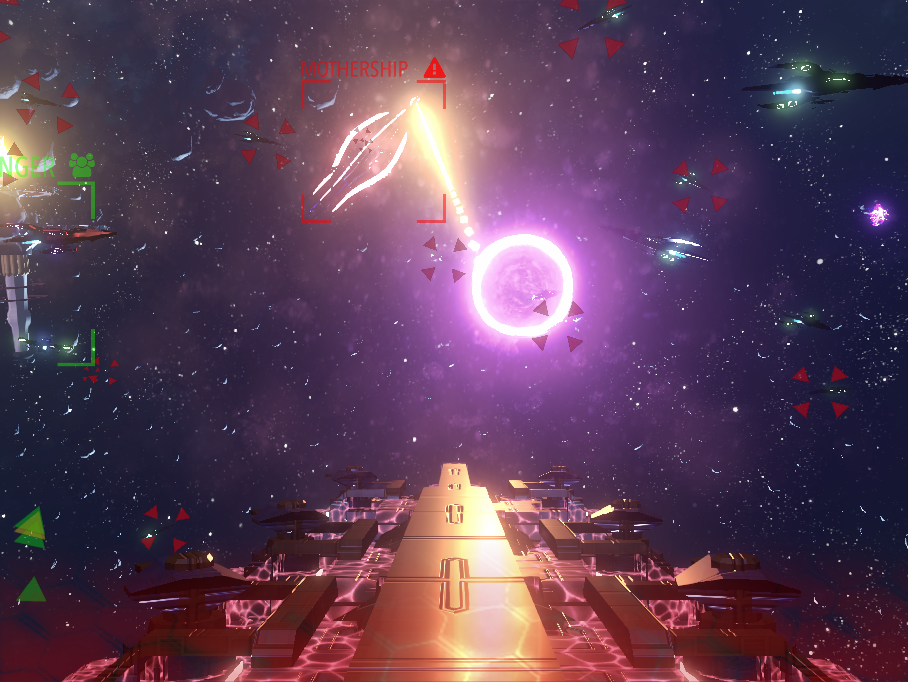
\includegraphics[width=.9\textwidth]{bloomOn}
        \captionof{figure}{Bloom enabled}
        \label{fig:bloomOn}
	\end{subfigure}
	\caption{Bloom effects}
	\label{fig:bloom}
\end{figure}

One of the most important visual effects in our game is the addition of real time volumetric lighting cast by the sun’s directional light. It is a very expensive effect and has only become feasible in real time graphics in the last couple of years. Without the effect applied, the scene is very bland and lacks depth. With the effect, objects such as the asteroids and enemies cast beautiful 3D shadows and it becomes easier to judge the distance of objects based on how \emph{foggy} they are. The effect parameters needed a lot of tweaking to get working in a space environment as it is typically used for sunlight rather than a completely open environment.

\begin{figure}[ht]
	\centering
    
    \begin{subfigure}{.5\textwidth}
      \centering
      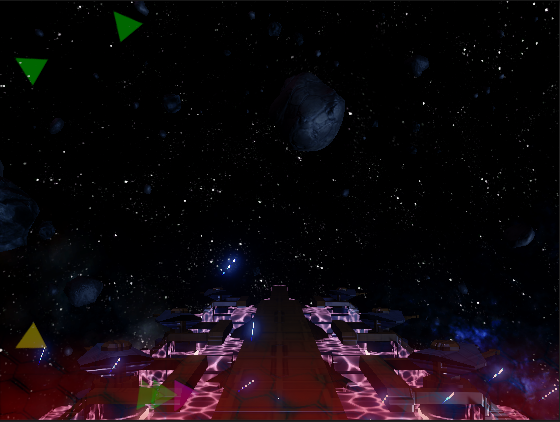
\includegraphics[width=.9\textwidth]{volumetricOff}
      \caption{Volumetric Lighting Disabled}
      \label{fig:volumetricOff}
    \end{subfigure}%
    \begin{subfigure}{.5\textwidth}
    	\centering
		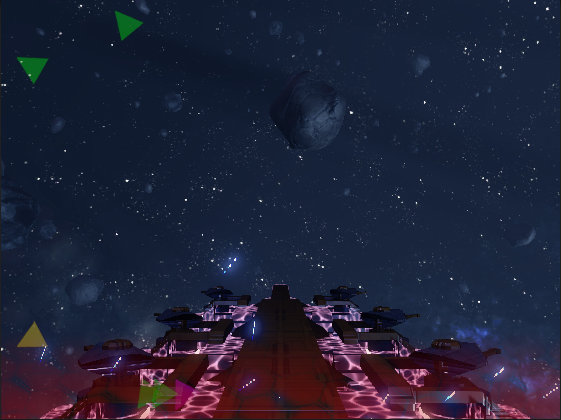
\includegraphics[width=.9\textwidth]{volumetricOn}
        \captionof{figure}{Volumetric Lighting Enabled}
        \label{fig:volumetricOn}
	\end{subfigure}
	\caption{Volumetric Lighting}
	\label{fig:volumetric}
\end{figure}

\clearpage

\section{Individual Contribution}

\subsection{Dillon Keith Diep}

\subsubsection{Main Game Logic and Networking}

Our team often challenged the most technical or uncertain problems first as a mean to de-risk. One of my early tasks was to investigate UNet framework and implement a foundation for other members to build upon. Many of our members had no prior experience with Unity Engine, while I was comfortable from past experience. Under these circumstances I stepped forward to tackle the initial networking and assisted others in familiarising themselves with the workflow of Unity Engine.

In addition to the core network communication, several significant sub-systems were developed by me. Our solution uses a custom lobby system required for setup phase of multiple clients with different roles, this was a prerequisite for aligning networked cameras. I also adapted initially single-player features such as the crosshair aiming and auto-targeting to support extra screens added as clients. I generally oversaw the game state transition over the network - providing a method for resetting the game efficiently and creating the tutorial diagrams presented during the pre-gameplay phase.

\subsubsection{Multiple Aligned Camera System}

The camera system depicted under the technical content section was implemented by me. I was keen on providing a scalable networked solution that could leverage computing power in parallel.  My solution to align view frustums was inspired by the pinhole camera model and theory acquired recently from COMS30121, the image processing and computer vision unit.

\subsubsection{Asset Production, Art \& Design}

Assistance in visualising the game through concept art and 3D asset production including the two enemy ships, engineer model, and mothership displayed under the technical content section.

\todo[inline]{Insert pictures}

\subsubsection{Others}

My role as the project manager required little effort as each member of the team was highly motivated. The primary intention as project manager was to direct the team forward - planning ahead to ensure smooth progression and avoid the need to clutch out near the end. Communication is vital, thus I often remained contactable at all times and aimed to respond to all enquiries within a day. The professional culture among our team secured a productive collaboration with the musicians and our mentor. In terms of general development I have contributed to a wide-spectrum of tasks. Due to my availability and experience with Unity, on many occasions I was able to provide support for my peers and push the project forward. To minimise issues that may hinder other members, I had also allocated considerable time to the investigating and resolving of critical bugs that have occurred.

\clearpage

\subsection{Frank Hemsworth}

IR Shooting Controller + IR LEDs
Physical Guns with mechanism for the trigger.
Initial Missions Functionality
Command Console Layout + Functionality
Room layout and design
Physical Networking
DNS Server
Stats Server
Player Scoring
Spectator Screen
Phone Game

Team management, task organisation and managing git repository

\clearpage

\subsection{Marc Steene}
Having already used the Unity engine for several years, my prior experience has allowed me to contribute to almost every part of the game in some way. My main focus throughout the project has been on graphics related tasks, along with the main game logic, networking, and heavy optimisation to maximise frame rate.

\subsubsection{Main Game Logic and Networking}
I have contributed to a large portion of the main game logic, including the player flying logic, shooting logic, collision detection, asteroid logic, damage effects, particle effects, ingame targets, and the Mothership logic.

On top of this, I have also been involved with networking game objects between the server and client, using both Unity’s built in network transform component as well as custom solutions using Remote Procedure Calls and Commands.

\subsubsection{Graphics}
Using Maya 2016 and the skills learned in the Character and Set Design unit, I created and textured the 3D models for the player ship and outposts. I was also responsible for texturing the enemies in Unity. 

Using Adobe Photoshop CS6, I created the team logo, game logo, and many of the 2D icons found in the game. The majority of the graphics are created in vector format, and Unity can import PSD files natively. This means that the icons will still be crisp if they need to be resized or when rendering to higher resolutions.

\begin{figure}[ht]
	\centering
	
\includegraphics[width=\textwidth]{images/2dArt}
\end{figure}

I set up the image post processing stack using both Unity’s built in shaders, as well as open source ones available on GitHub and tweaked them to be visually pleasing and coherent with one another.

\subsubsection{Optimisation}
I spent many hours optimising the game to run as smooth as possible on our target hardware. This included optimising the graphics by adjusting culling, implementing a level of detail system to reduce polygon count, and finding bottlenecks using Unity’s GPU profiler.

I was also in charge of optimising the game logic by finding clever techniques to reduce the CPU usage as much as possible, once again using Unity’s built in CPU profiler to find bottlenecks.

\clearpage

\subsection{Andrei Poenaru}

Most of my tasks involved the core game logic. While I had not worked with Unity before, by the end of the project I contributed code to most parts of the main game, including gameplay mechanics, interaction with networked component and general optimisations.

\subsubsection{Game AI}

I developed the enemy ships’ AI from the ground up. Inspired by a strategy for a fighter plane dogfighting AI, the system I implemented uses randomness to make enemy ships swarm the player in an unpredictable fashion. The code is optimised to use as few resources as possible, since there can be over 200 enemies active in the scene at any one time.

As part of the AI, I developed and obstacle avoidance strategy for the enemies. This uses the technique of \emph{raycasting} to check for obstacles ahead, and then to confirm they were successfully avoided. This system allows enemies to circle the player’s ship without colliding with it or other enemies, while also dodging asteroids and moving around larger structures like outposts or the Glom Mothership.

The enemies can also be \emph{hacked} through the spectator game. While hacked, enemies can be commanded to move to a certain position, follow the player, or attack a chosen target. I have implemented all of these behaviour options using the AI’s framework.

\subsubsection{Weapons system}

Another important component I developed was the ability to shoot. With data provided by the IR sensors, I have implemented all the logic that displays the aiming position through a crosshair, positions the turrets to the right positions, then fires bullets. I have also implemented a rechargeable ammo system, which prevents the players from constantly firing by regenerating ammo slower than the firing rate. To implement the shooting damage, I designed the collision logic for most objects in our game, including asteroids, enemy ships, the player’s ship, and large structures such as outposts.

Because aiming proved to be difficult due to crosshair jitter, I have implemented \emph{smoothing} by using interpolation, and an aim assist system that locks the crosshair onto nearby enemies. The latter proved vital to achieving good shooting accuracy.

\subsubsection{Object spawning and clean-up}

I have implemented most logic for spawning and despawning objects in our game. This covers creating enemies as needed, initialising outpost guards, asteroids, and asteroid fields. This latter part proved to be fairly difficult because a balance had to be found between having enough asteroids around the player to maintain immersion, while also not using too many resources for asteroids further away. I also implemented code that cleans up all the spawned objects when preparing for a game restart.

\subsubsection{Upgradable components}

I developed most of the backend logic that allows ship components to be damaged and upgraded. While not in charge of the UI, I made upgrades possible through a clean, object-oriented framework.

\clearpage

\subsection{Luke Bryant}

\subsubsection{Command Console}

The largest part of my contribution was on developing the command console. I wrote a large proportion of the logic code for this part of the game, created almost all of the 2D graphics, and was responsible for making sure that the command console presented the player with all the information that the commander needed, while ensuring they were not overwhelmed by features. This was perhaps the most complicated part of the game for the user, so an approach of continual user-testing and UI adjustment was necessary for every UI element. For example, each “ship component” button needed to be quite compact and aesthetically pleasing, but show the name of the component, the current component level, whether an upgrade was pending, the damage sustained by the component, whether a repair was pending, the cost of the next upgrade (as well as color cues to show affordability) and buttons to request upgrades and repairs. Other time-consuming UI elements which I implemented include the strategic map, ability buttons and various mission-related UI elements. I also implemented some of the networking between the command console and the main game.

\subsubsection{Missions}

I contributed a large amount of code towards the mission logic in the game by adding more features to the substantial base code that was produced by Frank Hemsworth. This included adding visual indication of objectives, both on the main game and on the command console; increasing the variety of mission conditions and triggers that could be used, and ensuring flexibility and customisation potential in the missions system, so that the number of missions and their parameters could be easily modified in the light of feedback and new design decisions. The wide range of possible mission parameters meant that they needed a substantial amount of testing and bug fixing, across the whole networked unity game, which I was largely responsible for.

\subsubsection{Stats Screen}

We decided to broadcast game statistics that might be interesting to the spectators during the game to a web page which would be displayed on a large screen facing the spectator section. In order to do this, I set up a unity client which would communicate current game statistics to a Go server, which I also wrote. Additionally, I implemented the functionality for the Go server to store data in an SQL server which could store game statistics. Finally, I set up a web page displaying the chosen statistics, which was hosted by the Go server, including graphical assets.

\subsubsection{Main Game}

It was noted early on that navigation in space could be confusing and players could be easily disoriented. To address this problem I developed indicator arrows in different colours that would point to various landmarks that were relevant to the game’s progression. I used a trigonometric approach to ensure that any landmarks that were not seen by the central camera had corresponding UI arrows that would point off-screen to them. I also implemented this system on the engineer console to guide the engineer back to the ship if they strayed too far from it. Additionally, I dealt with various smaller miscellaneous features and bugs that arose on the main game.

\clearpage

\subsection{Stoil Ganev}

\subsubsection{Phone Server}

The majority of my work on this project was dedicated to the Phone Server component of the game. I built it from scratch using the Go programming language. I chose Go since it has a simple approach to concurrency. One of my aims with this server was to make it scalable in terms of the number of clients it can handle at any time. I achieved this by adopting an easily scalable multithreaded design and constructing data structures that allowed thread-safe concurrent access.

A key feature of the Phone Server is its reliable connection to the Game Server. I implemented the majority of the message passing between the two components. This involved placing reliability and automatic reconnection measures in place as well as designing the message structure. The final design of the messages was inspired by the TCP/IP Network stack in the sense that each message wa comprised of multiple layers specifying the type of data it carries. This allowed us to easily parse the messages as well as to easily extend any layer to allow for more types of messages to be handled. I constructed the message passing interface around an easy to use API that allowed any team member to easily modify it.

Another aspect of the Phone Server was the proper handling of user connections and user input. Due to the unpredictable nature of users, I had to conduct a lot of rigorous testing. This helped me identify a significant amount of edge cases that I often overlooked. This process continued throughout the year and especially when a big change was made in the overall system.

Due to the nature of the phone clients, some amount of preprocessing of the game data has to be done on the Phone Server before it can be sent to them. The positional data of the game objects received from the Game Server is based in the 3D view of the game engine. However, the phone clients need a 2D projection of this world that is easily understandable by users. To construct this view I made use of an orthogonal projection of the game objects onto a plane that is parallel to the player ships forward and right directions. This allowed me to achieve a top-down \emph{minimap} view of the world around the ship.

\subsubsection{Spectator Game}

The spectator game was one of my other major involvements. As mentioned above it was based around Pixi.js, however that simply provided a foundation for the rendering and all work related to scheduling frames and scaling and positioning of sprites still had to be done. From the ground up I build the rendering system to easily adapt to any size screen and resize objects when necessary. Once this was in place I proceeded with adding some simple animations and introducing an user interface.

\clearpage

\subsection{Artur Gemes}

\subsubsection{The Engineer Game}

I was the main developer of the engineer game. This meant that I was responsible for implementing the gameplay, and any networking required by the engineer. In fact, almost all of the implementation was done by me, except for some minor tweaks, and some graphical effects that were done by Marc Steene, and Luke Bryant.

From the beginning it was agreed within the group that the engineer game would be a first person experience. Therefore I developed the engineer game in an FPS (First Person Shooter) style. This meant that a lot of the design decisions were predetermined, such as decision of the movement controls. For example, using WASD as the keyboard movement controls has been the De facto standard in FPS games for many years now. I began by developing a simple single player demo for the engineer game. It had only the movement implemented, and an initial design of how the user would interact with ship components. The interaction with ship components is done by performing a raycast from the engineer. When this ray hits a ship component the engineer checks whether any interaction with the component is possible. If yes then the user is prompted to perform the interaction. This simple demo was useful as it gave the rest of the team an idea early on about what the engineer game would be like, and it also aided development as I could integrate often and see how the game was progressing.

To make the engineer feel more like a remote drone we decided that it would be controlled via some sort of joystick controls. Initially we were going to use an Xbox 360 controller. I implemented the Xbox controls, however shortly after we acquired a Saitek X52 flight system. This was a two joystick setup that is mostly used for flight simulators. Luckily interfacing with the new controller was made easy but Unity’s input manager, and I created a draft of the controls so that we could test the Saitek X52 against the Xbox 360 controller. In the end we decided to go with the X52, so I finalised the input mappings for it.

\subsubsection{Networking}

As the engineer was designed to be a remote client I was involved in the networking from early on. I participated in researching, designing and implementing all iterations of our network. In particular I designed and implemented a message passing framework that allowed clients to send messages to other clients specifically, using the server to route the messages. This involved researching and using Unity’s lower level networking API, as the high level API currently only supports broadcasting from the server to all clients. The motivation for doing this was reducing network load, as it reduced the number of broadcasts across the network. I also provided a network API for other parts of the game, so that other members of the team could easily communicate necessary data to the server using the API calls I implemented.

\subsubsection{Phone Game}

I had a small involvement in developing the phone game. I implemented some of the enemy hacking logic, and also some of the back end processing for the officer screen using Javascript. I also made small extensions to the admin panel, and the communication between the phone server and the main game server.

\begin{thebibliography}{9}

\bibitem{wiibrew_wiimote}
  Wii Remote,
  \url{http://wiibrew.org/wiki/Wiimote}

\bibitem{unity_camera}
  Unity Camera Class,
  \url{http://docs.unity3d.com/Manual/class-Camera.html}
  
\bibitem{unity_frustum}
  Understanding View Frustum,
  \url{http://docs.unity3d.com/Manual/UnderstandingFrustum.html}

\bibitem{frustum_equations}
  The Size of the Frustum at a Given Distance from the Camera,
  \url{http://docs.unity3d.com/Manual/FrustumSizeAtDistance.html}

\bibitem{html5_canvas}
  HTML5 Canvas,
  \url{http://www.w3schools.com/html/html5_canvas.asp}

\bibitem{pixi_js}
  Pixi.js,
  \url{http://www.pixijs.com/}

\end{thebibliography}

\end{document}